\section{Simulations}

\subsection{Outer loop}
\begin{frame}[fragile]{Outer loop: Tracking  }
  \textbf{Trajectory tracking of \textsl{cubic polinomial trajectory}} with $t\in[0,T]$\\
  \bigskip
  \bigskip
  \bigskip
  \begin{columns}
    \column{.6\textwidth}
   \textbf{Initial values:}\\
    \smallskip
    \begin{tabular}{c c c}
      \toprule
      Variable & Value & Description \\
      \midrule 
      $\tilde{x}_{1,0}$  & $ 2 $ m & $x$ \\
      $\tilde{x}_{2,0}$  & $3$ m & $y$ \\
      $\tilde{x}_{3,0}$  & $4$ m & $z$ \\
      $\tilde{x}_{4,0}$  & $0$ m/s & $\dot{x}$ \\
      $\tilde{x}_{5,0}$  & $0$ m/s & $\dot{y}$ \\
      $\tilde{x}_{6,0}$  & $0$ m/s & $\dot{z}$ \\
      \bottomrule
    \end{tabular}
    \column{.4\textwidth}
    \textbf{Final values:}\\
    \smallskip
    \begin{tabular}{c c}
      \toprule
      Variable & Value \\
      \midrule 
      $\tilde{x}_{1,T}$  & $0$ m \\
      $\tilde{x}_{2,T}$  & $0$ m \\
      $\tilde{x}_{3,T}$  & $0$ m \\
      $\tilde{x}_{4,T}$  & $0$ m/s \\
      $\tilde{x}_{5,T}$  & $0$ m/s \\
      $\tilde{x}_{6,T}$  & $0$ m/s \\
      \bottomrule
    \end{tabular}
  \end{columns}
\end{frame}



\begin{frame}[fragile]{Outer loop: Tracking}
  \textbf{Trajectory tracking of \textsl{cubic polinomial trajectory}} with $t\in[0,T]$\\
	\begin{figure}[h]
	\centering
	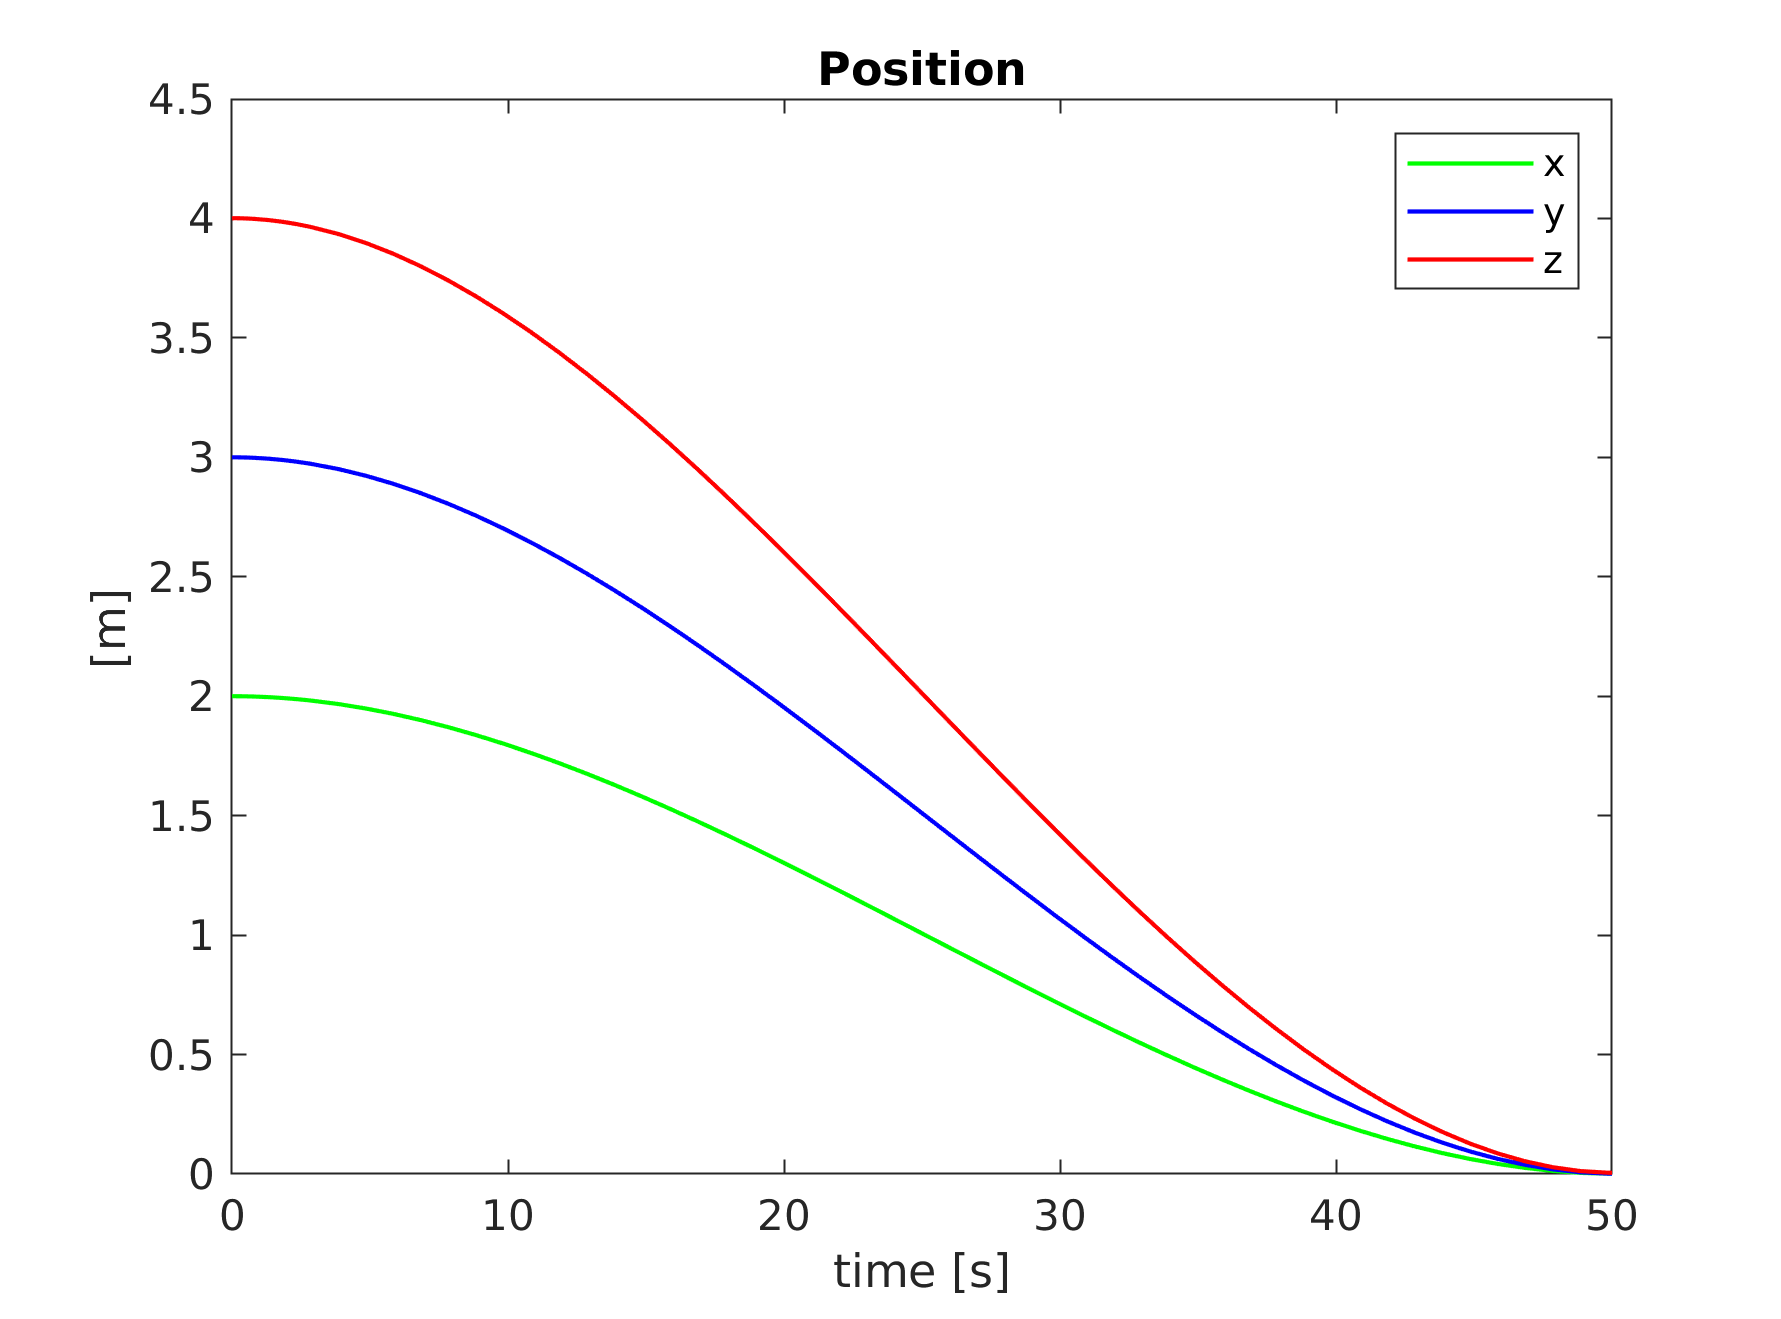
\includegraphics[width=0.93\linewidth]{../report/Images/PositionOuter}
	\end{figure}
\end{frame}

\begin{frame}[fragile]{Outer loop: Tracking }
  \begin{center}
  \textbf{Output of the \textsl{outer loop}:}\\
  $y_1 = \phi, \qquad y_2 = \theta, \qquad y_3 = r$
  \end{center}
  \begin{columns}
    \column{0.55\textwidth}
    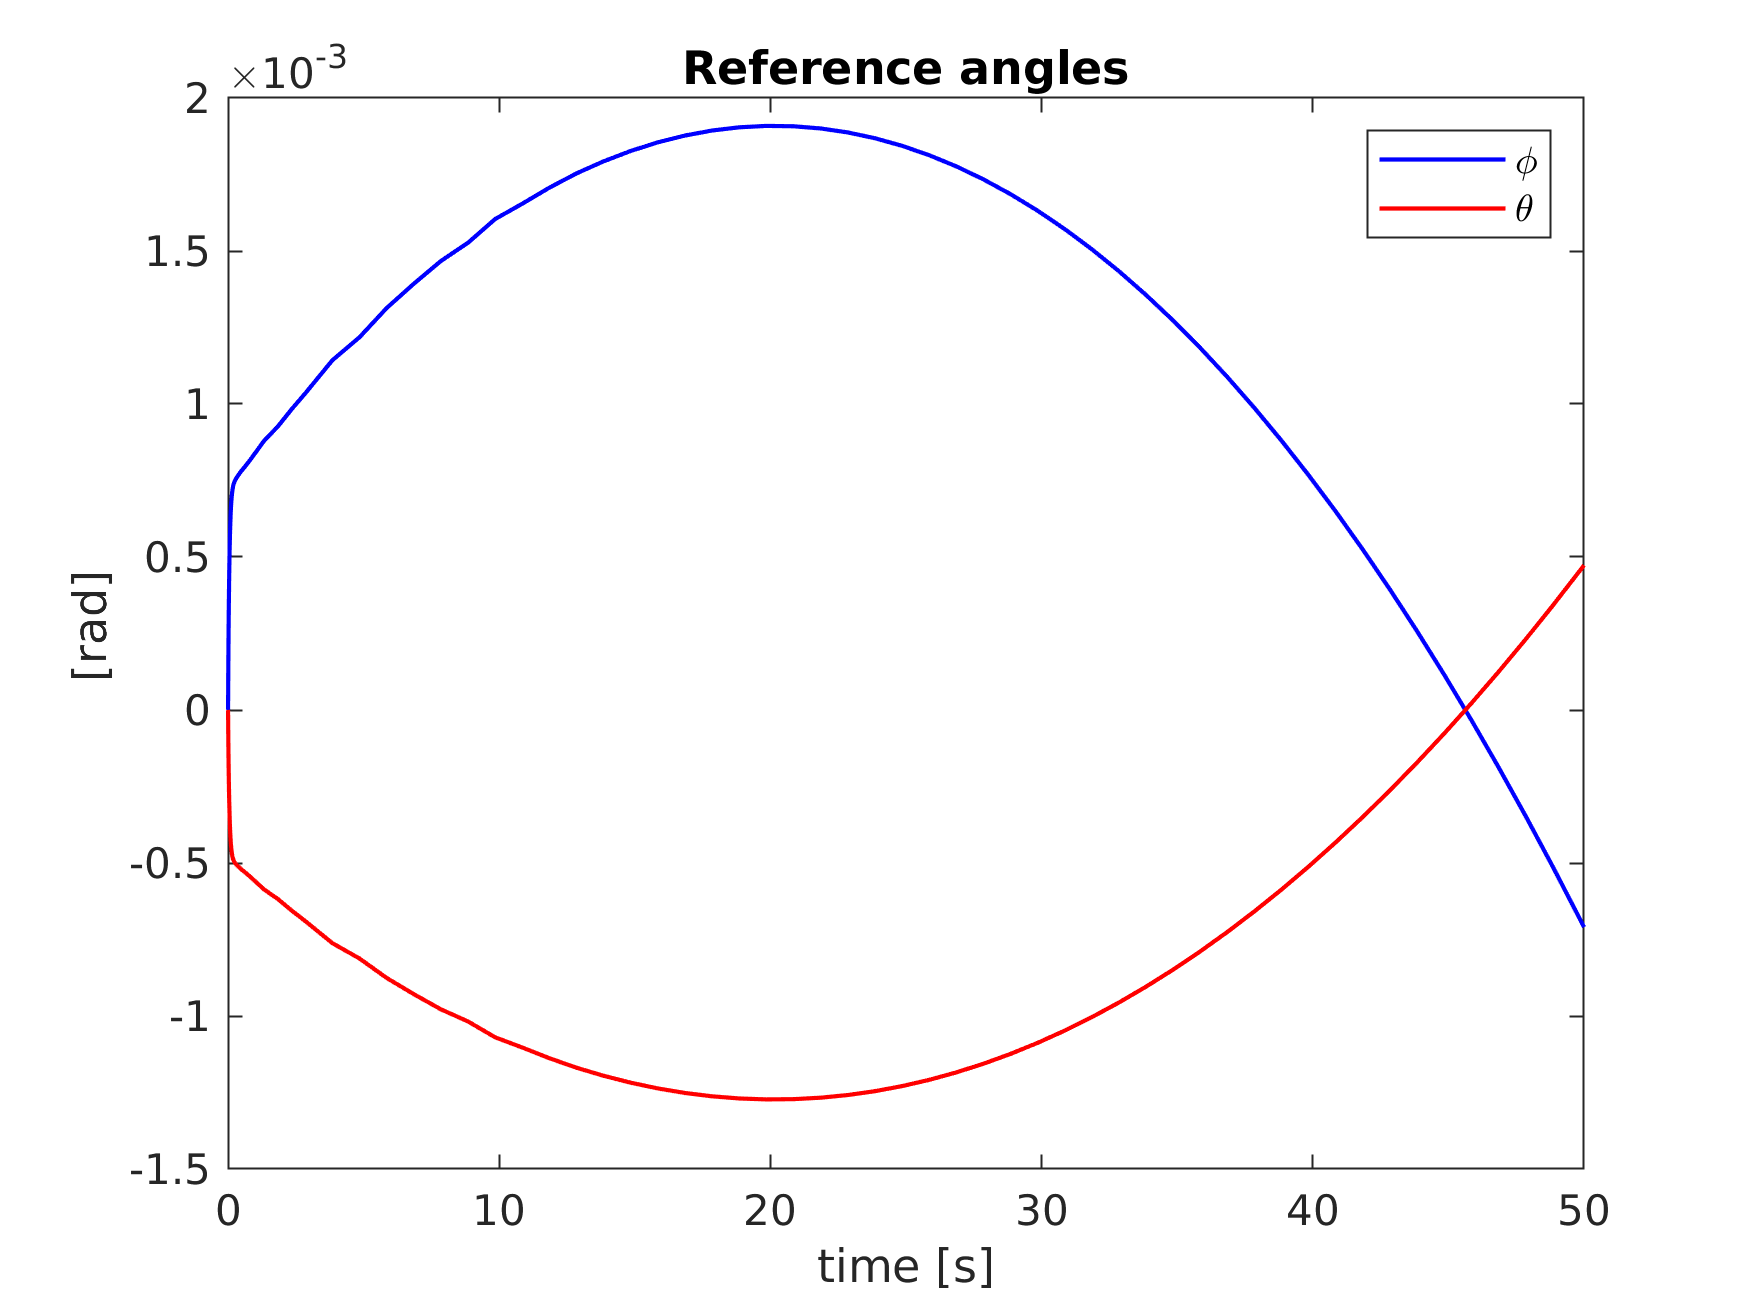
\includegraphics[width=\linewidth]{../report/Images/AngleOuter}
    \column{0.55\textwidth}
    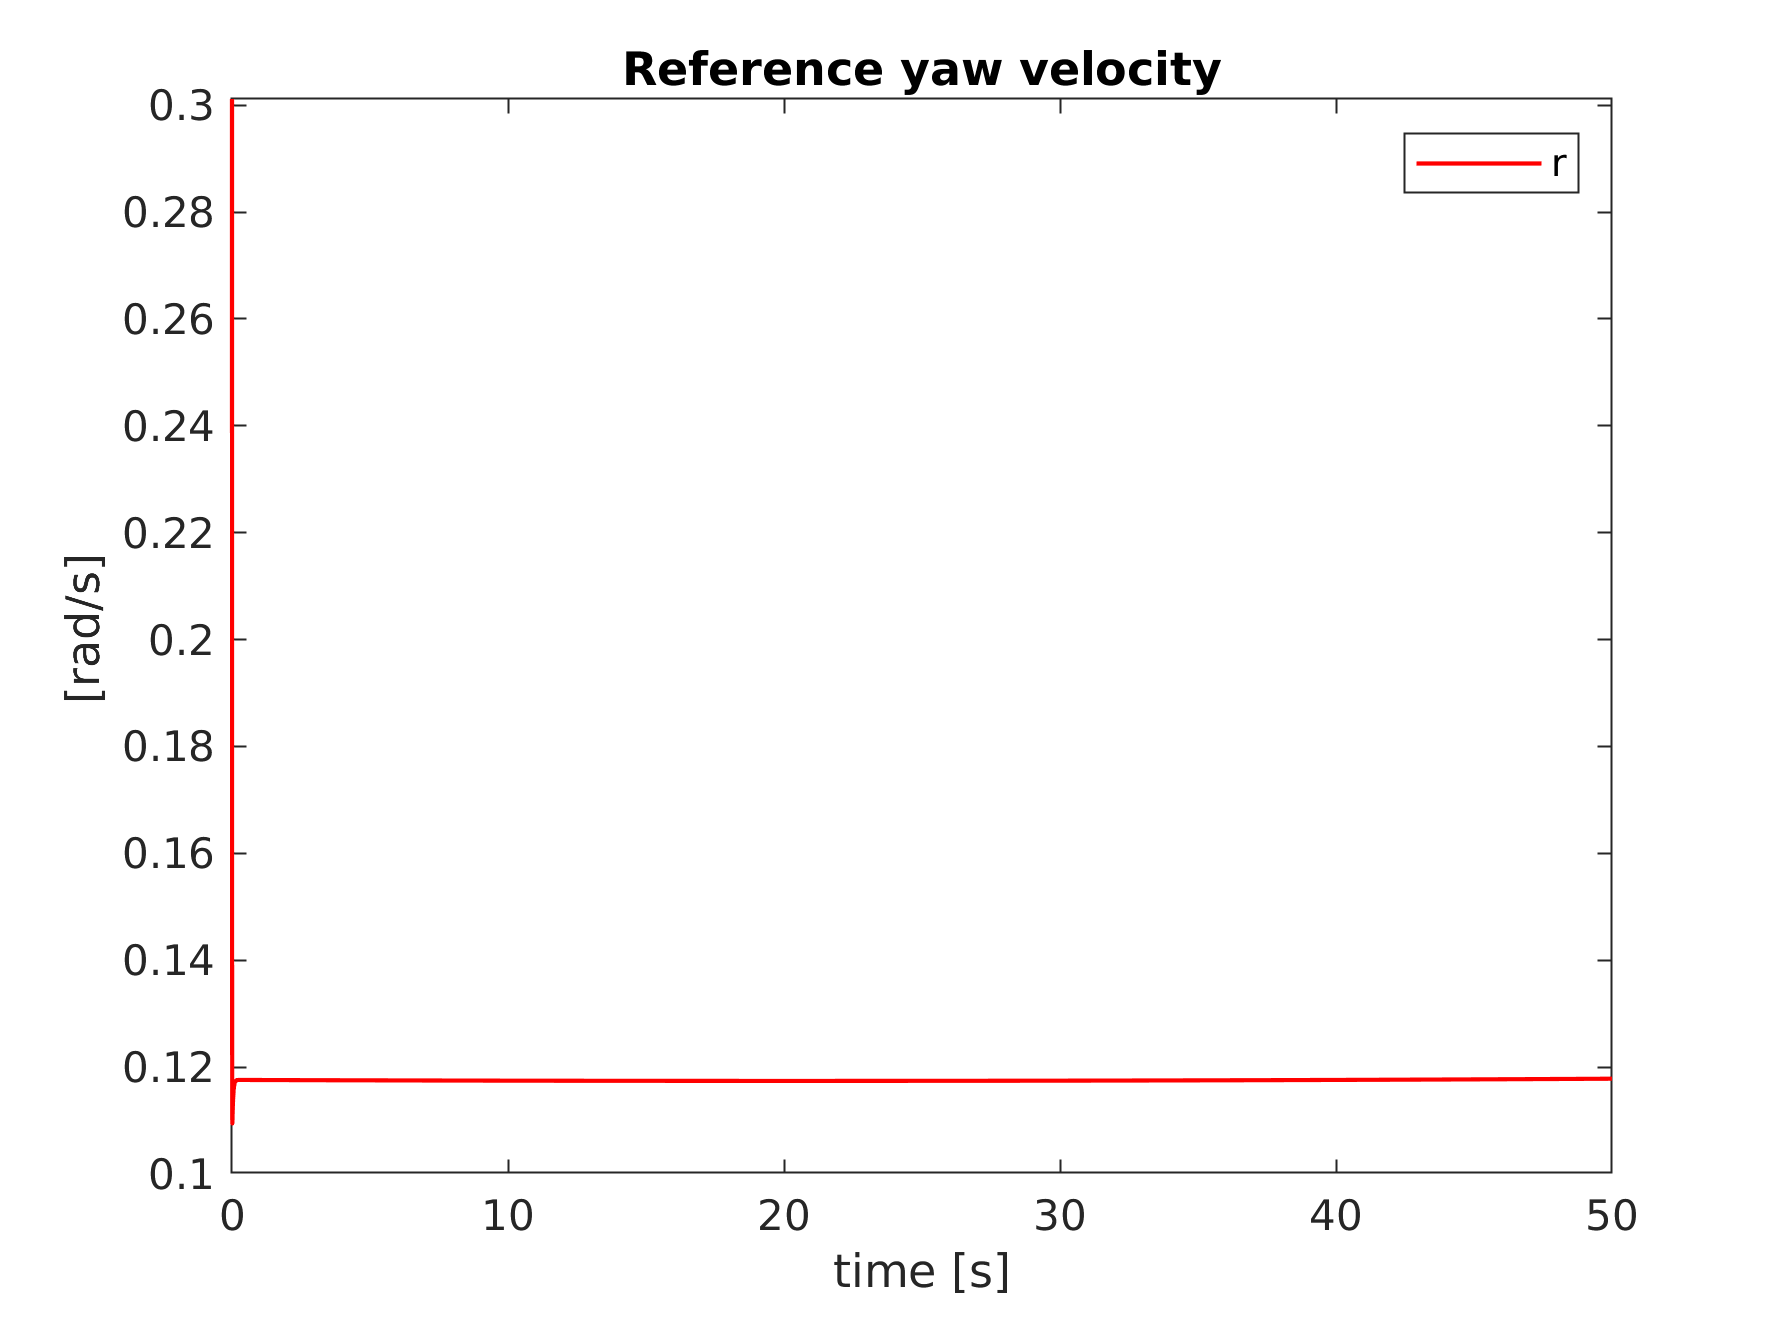
\includegraphics[width=\linewidth]{../report/Images/velOuter}
  \end{columns}

\end{frame}

% \begin{frame}[fragile]{Outer loop: Regulation}
%   \smallskip
%   \begin{columns}
%     \column{0.25\textwidth}
%     \textbf{Regulation task}:\\
%     more abrupt behaviour than in trajectory tracking.
%     \column{0.40\textwidth}
%     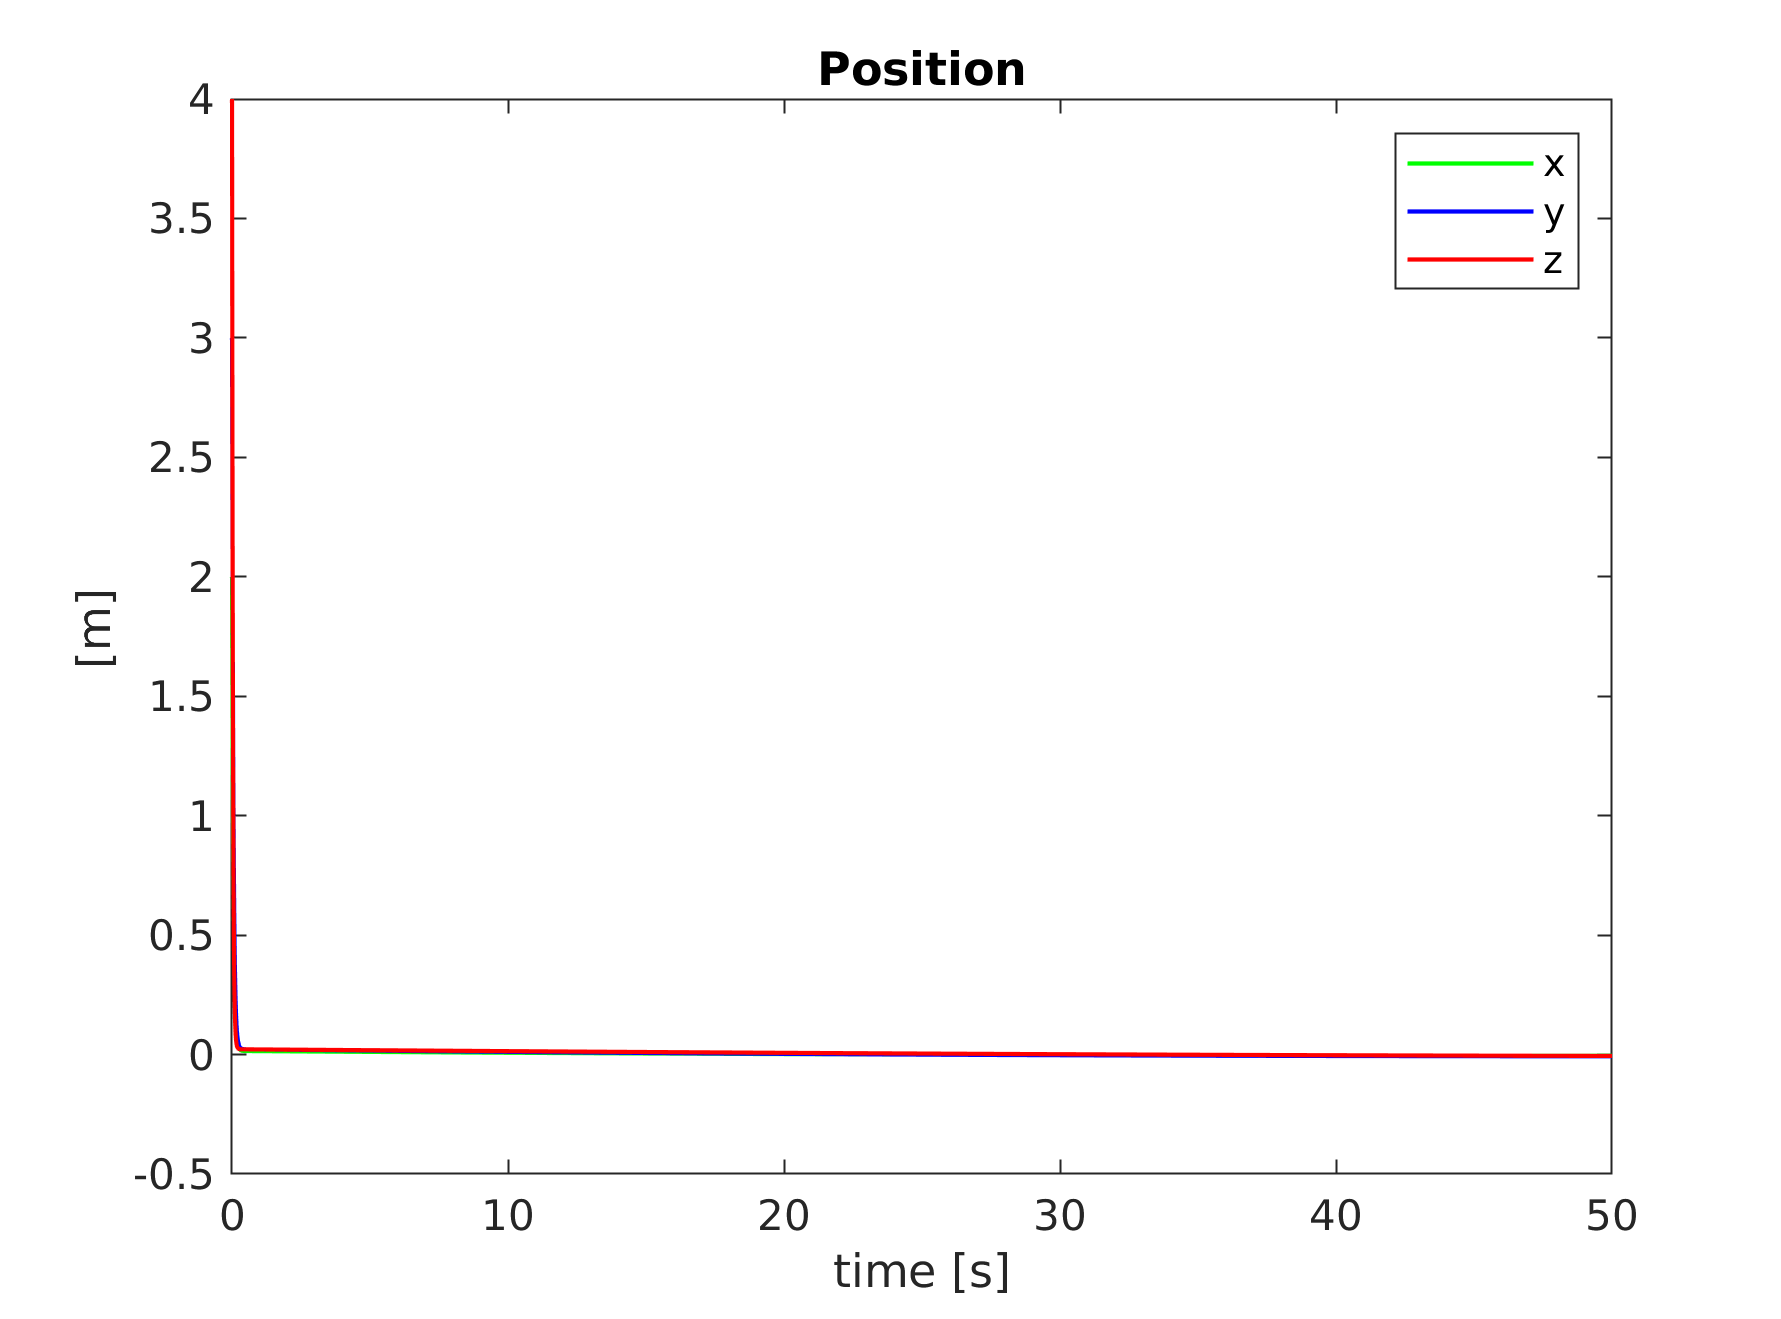
\includegraphics[width=\textwidth,
%     height=\textwidth]{../report/Images/PositionOuterNO}
%   \end{columns}
%   \begin{columns}
%     \column{0.4\textwidth}
%     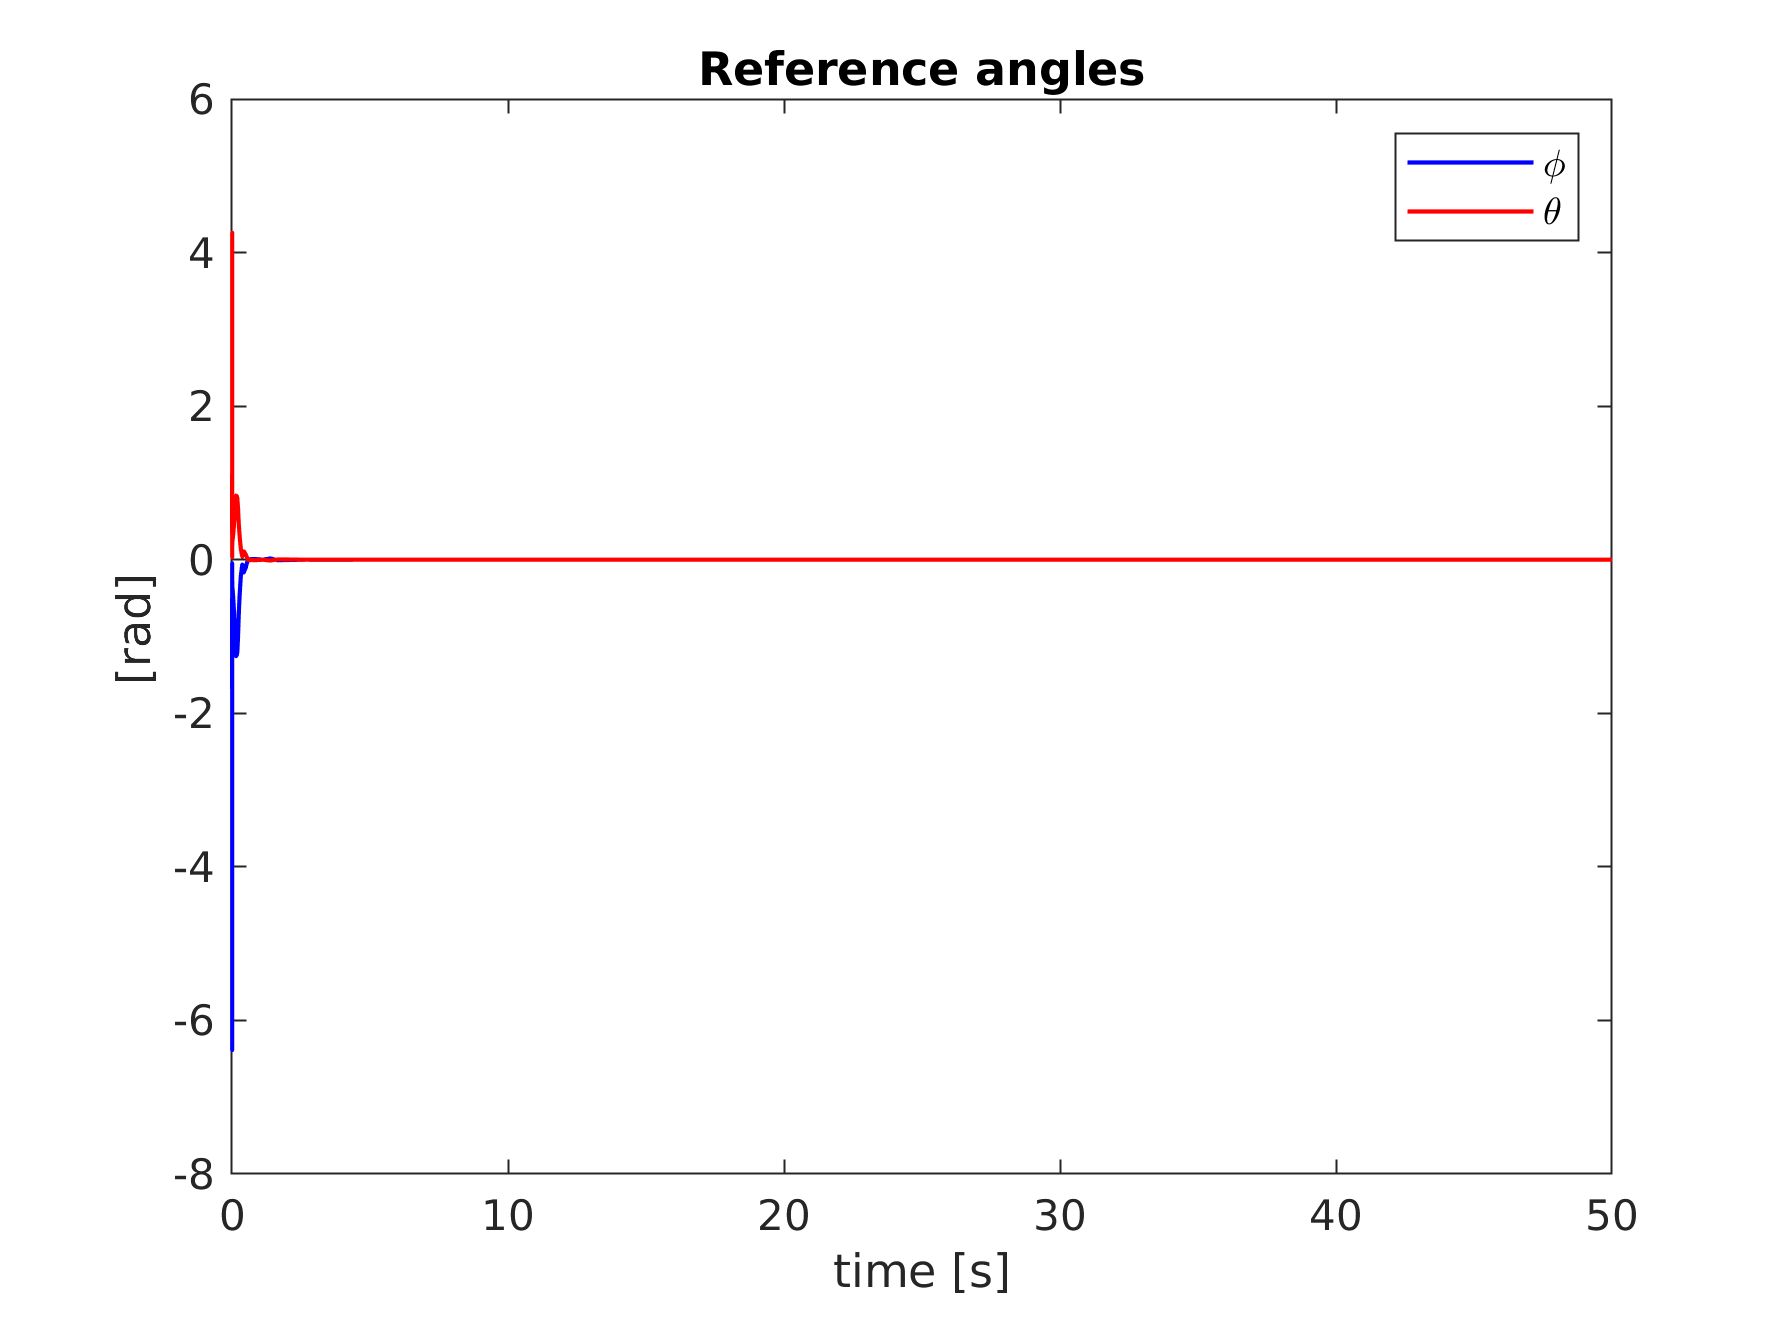
\includegraphics[width=\textwidth,
%     height=\textwidth]{../report/Images/AngleOuterNO}
%     \column{0.4\textwidth}
%     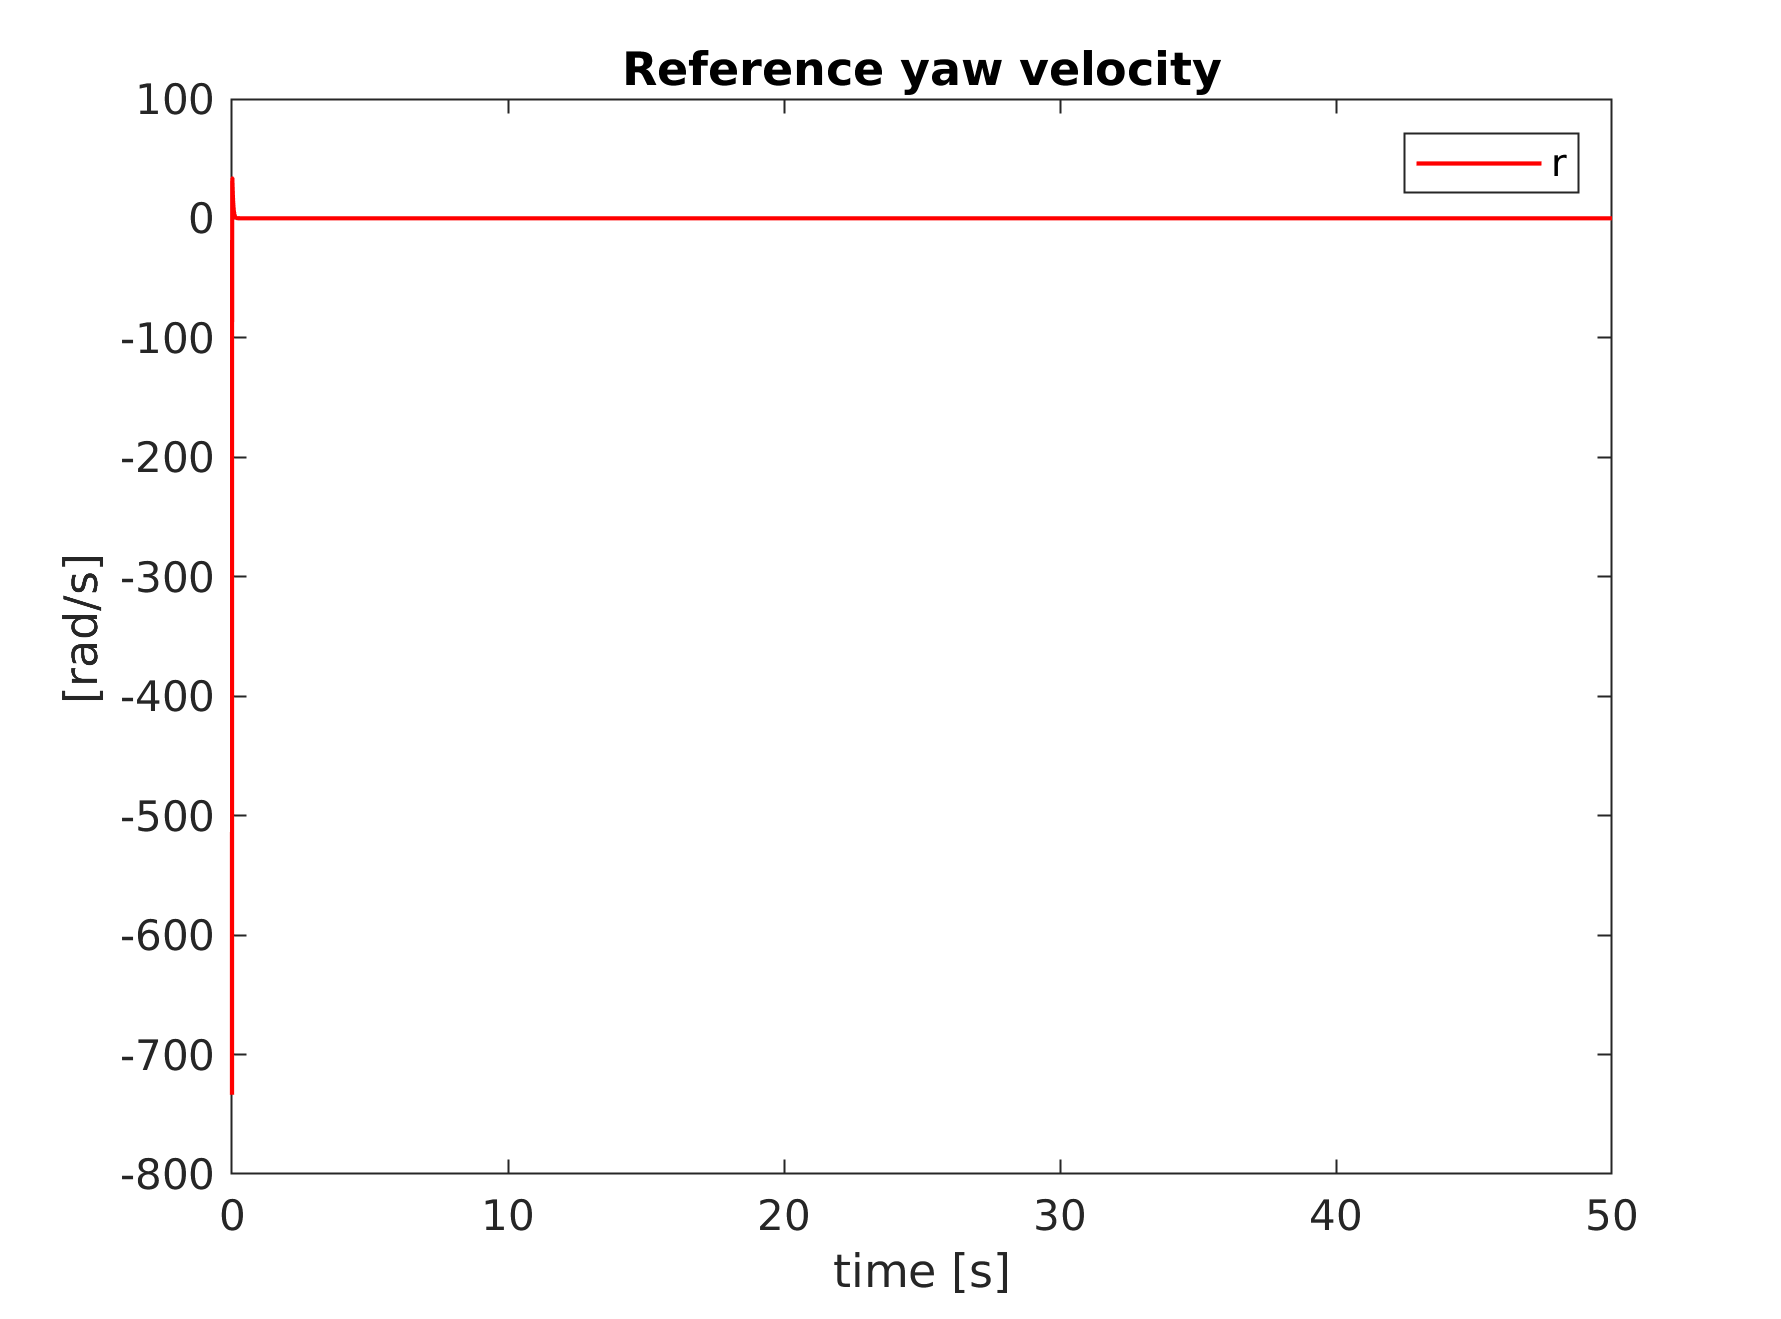
\includegraphics[width=\textwidth,
%     height=\textwidth]{../report/Images/velOuterNO}
%   \end{columns}
% \end{frame}

\subsection{Inner loop}

\begin{frame}[fragile]{Inner loop: regulation}
 \begin{columns}
    \column{.6\textwidth}
   \textbf{Initial values:}\\
    \smallskip
    \begin{tabular}{c c c}
      \toprule
        Variable & Value & Description \\
        \midrule 
        $x_1$  & $-\pi/4$ rad & $\phi$ \\
        $x_2$  & $\pi/4$ rad & $\theta$ \\
        $x_3$  & $\pi/4$ rad & $\psi$ \\
        $x_4$  & $-0.5$ rad/s & $p$ \\
        $x_5$  & $0.5$ rad/s & $q$ \\
        $x_6$  & $2.7$ rad/s & $r$ \\
        \bottomrule
      \end{tabular}
    \column{.4\textwidth}
    \textbf{Final values:}\\
    \smallskip
    \begin{tabular}{c c }
        \toprule
        Variable & Value \\
        \midrule 
        $x_1$  & $0$ rad \\
        $x_2$  & $0$ rad \\
        $x_3$  & $0$ rad \\
        $x_4$  & $0$ rad/s \\
        $x_5$  & $0$ rad/s \\
        $x_6$  & $mgd/k_r$ rad/s \\
        \bottomrule
     \end{tabular}
  \end{columns}
 \end{frame}


\begin{frame}[fragile]{Inner loop: Regulation}
  \begin{columns}
    \column{.55\textwidth}
    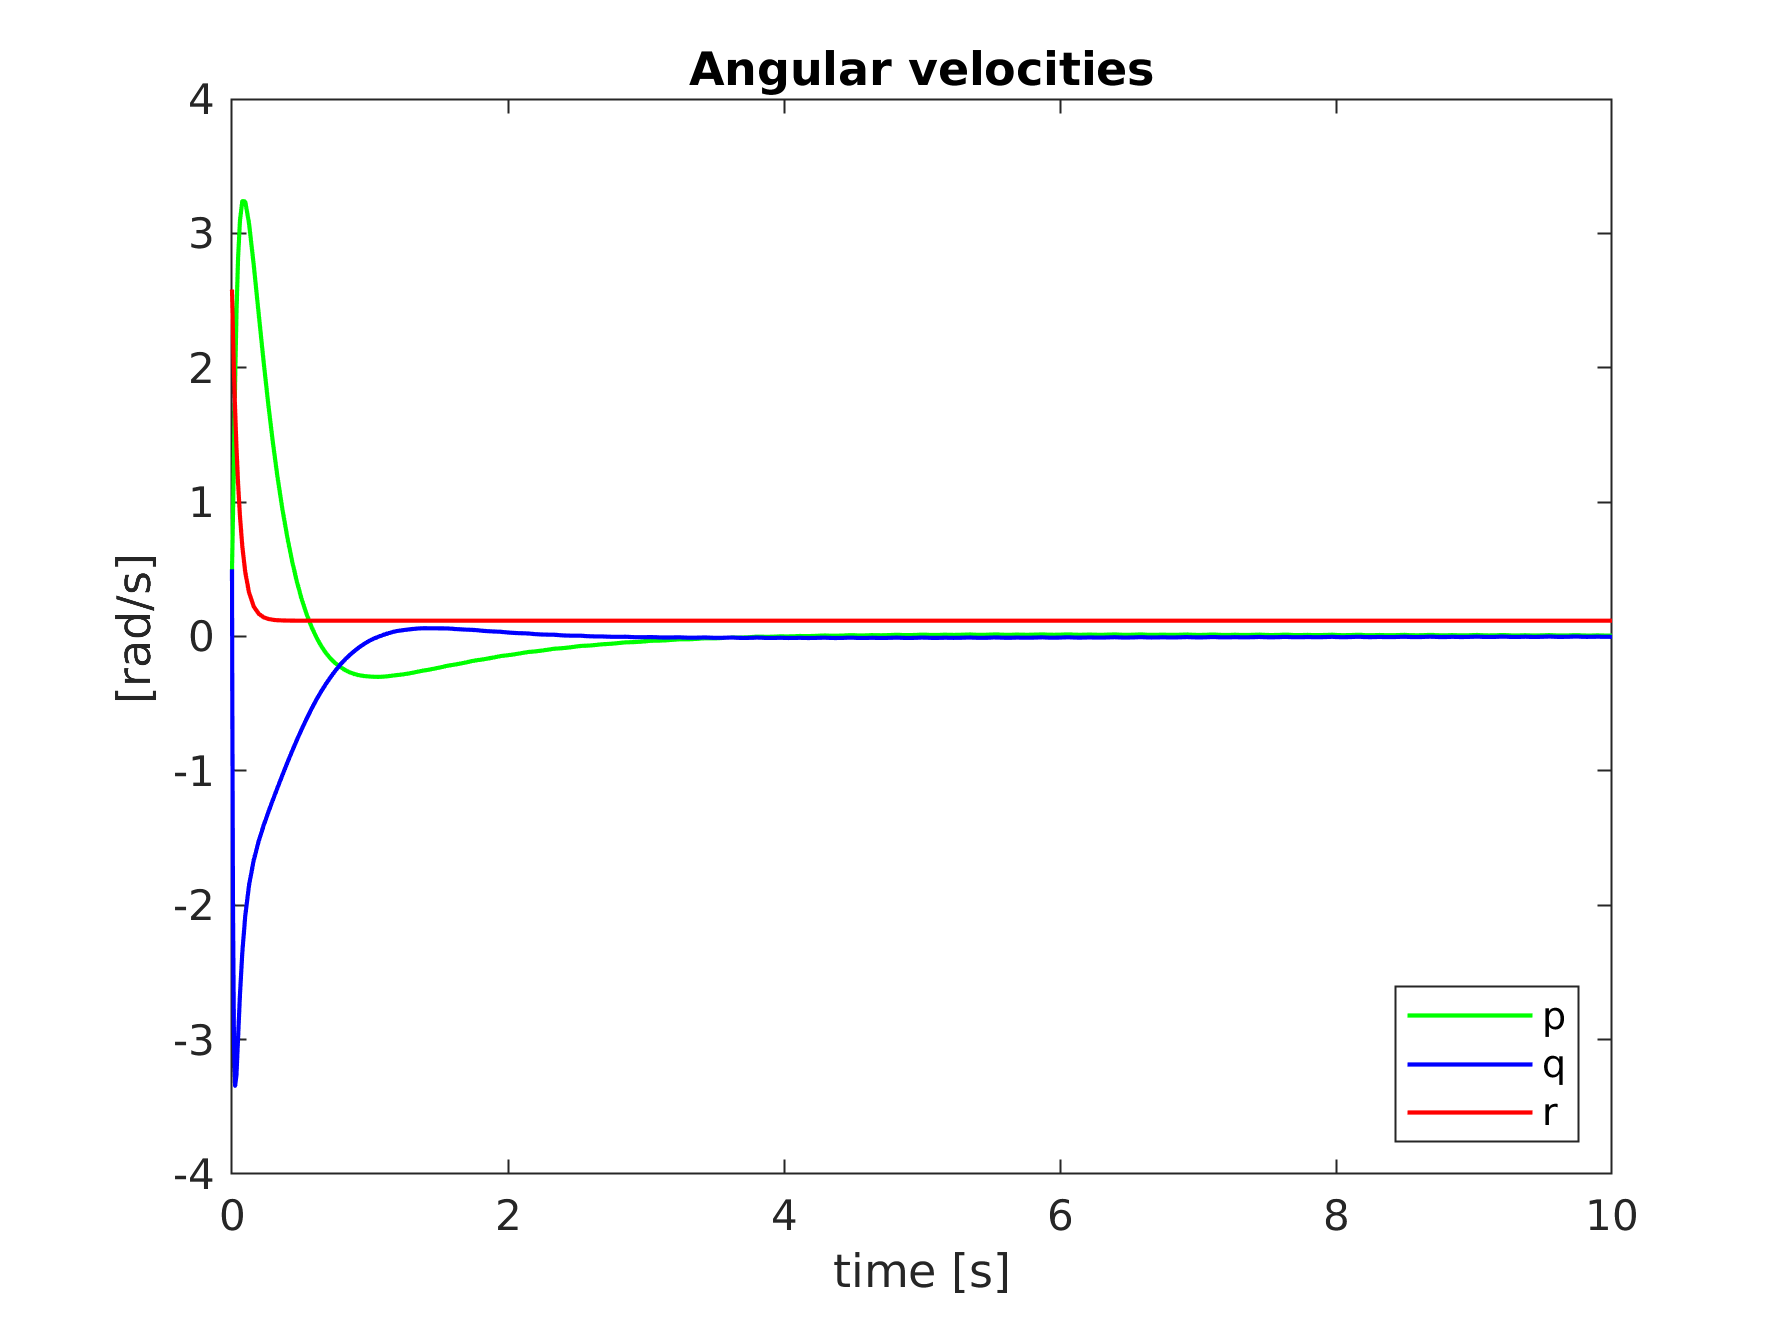
\includegraphics[width=\textwidth]{../report/Images/innerControlVel}
    \column{.55\textwidth}
    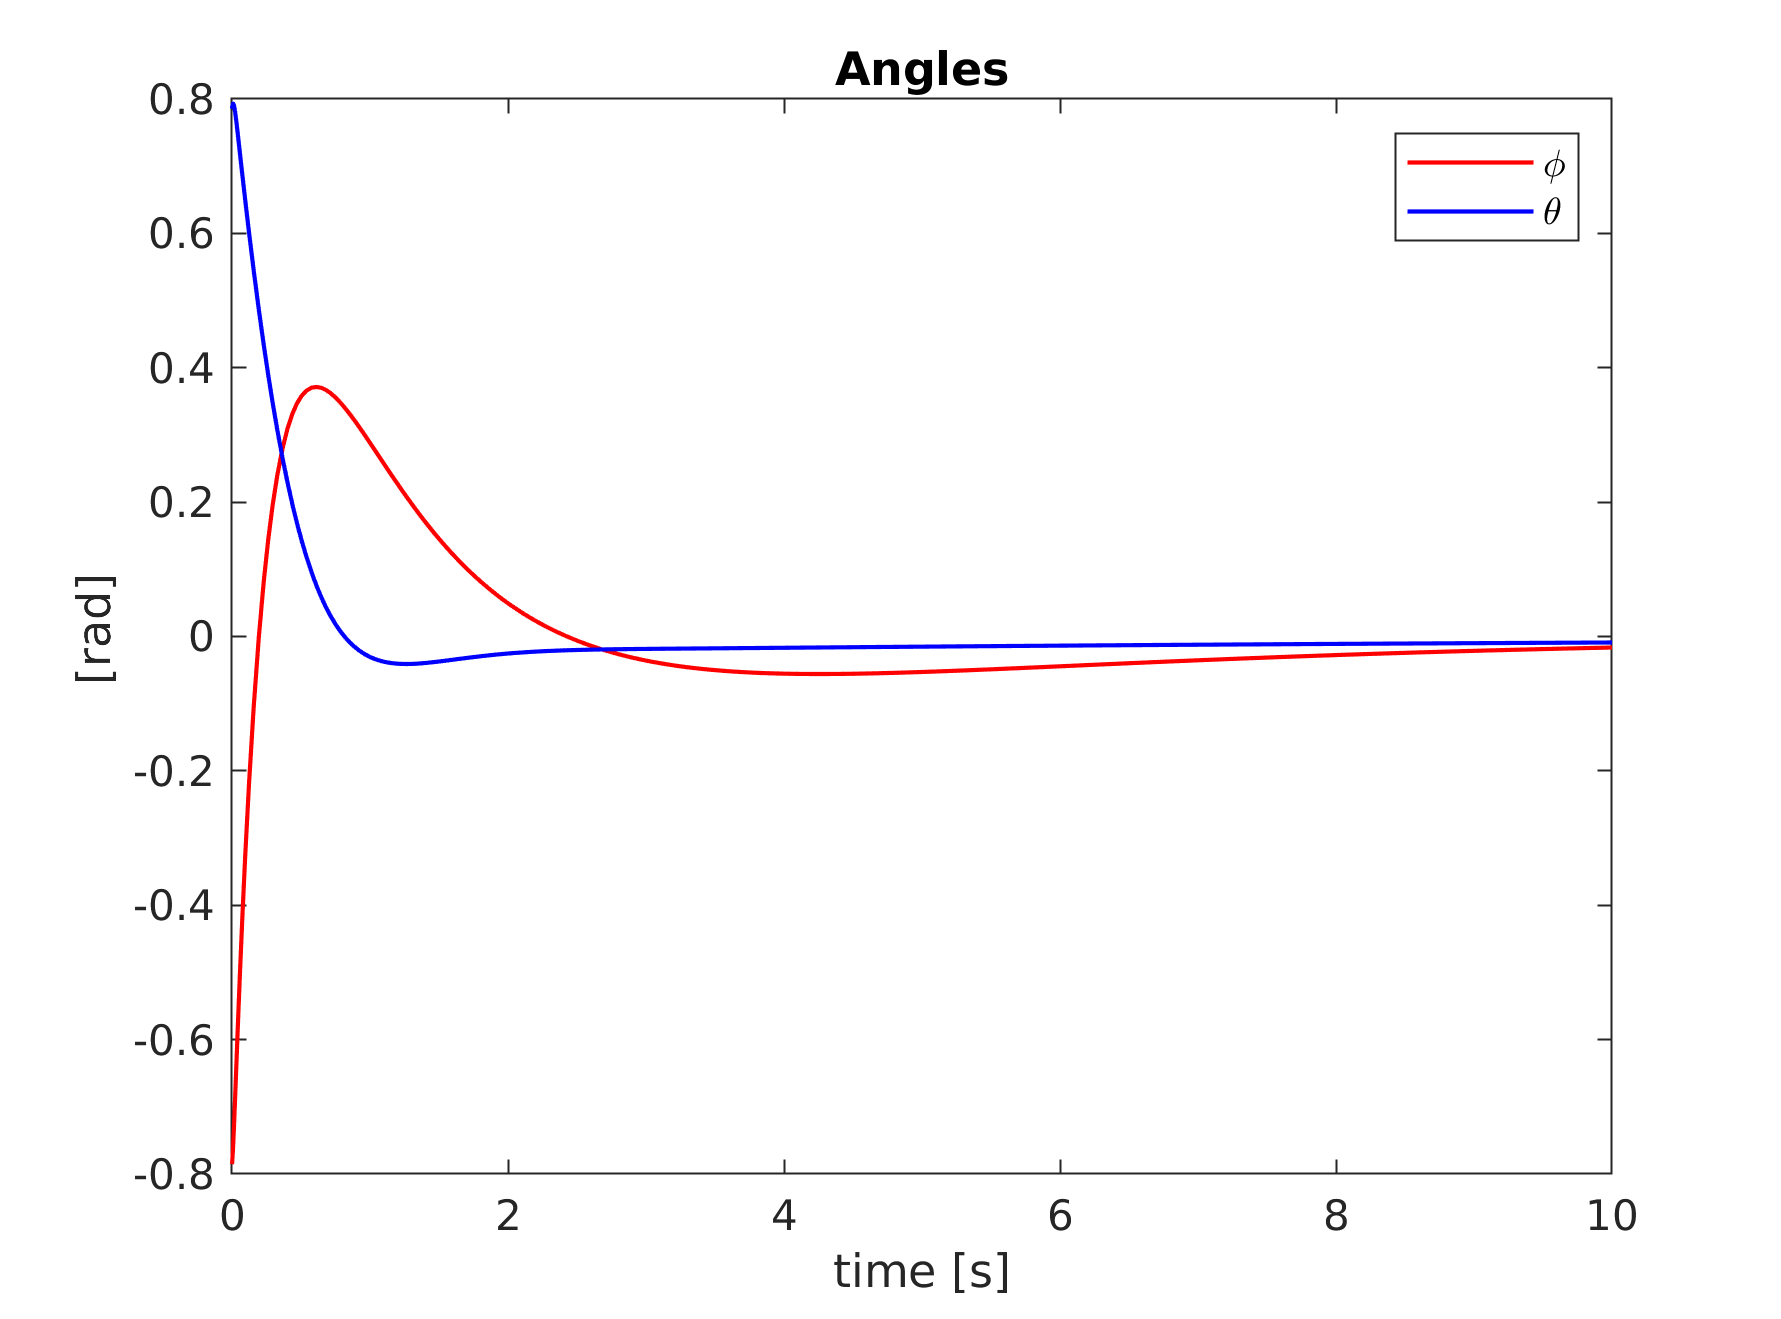
\includegraphics[width=\textwidth]{../report/Images/innerControlAngles}
  \end{columns}
\end{frame}

\begin{frame}[fragile]{Inner loop: Regulation}
    \includegraphics[width=\textwidth]{../report/Images/Forcesinner}
\end{frame}


\subsection{Complete loop}

% \begin{frame}[fragile]{Complete loop: regulation}
%   \textbf{Initial values:}\\
%   \smallskip
%   \begin{tabular}{c c c}
%     \toprule
% 		Variable & Value & Description \\
% 		\midrule 
% 		$x_1$  & $0.1$ rad & $\phi$ \\
% 		$x_2$  & $-0.1$ rad & $\theta$ \\
% 		$x_3$  & $0.1$ rad & $\psi$ \\
% 		$x_4$  & $0.2$ rad/s & $p$ \\
% 		$x_5$  & $-0.2$ rad/s & $q$ \\
% 		$x_6$  & $0.15$ rad/s & $r$ \\
% 		$x_7$  & $5$ m & $x$ \\
% 		$x_8$  & $5$ m & $y$ \\
% 		$x_9$  & $5$ m & $z$ \\
% 		$x_{10}$  & $0$ m/s & $\dot{x}$ \\
% 		$x_{11}$  & $0$ m/s & $\dot{y}$ \\
% 		$x_{12}$  & $0$ m/s & $\dot{z}$ \\
% 		\bottomrule
%   \end{tabular}
% \end{frame}


\begin{frame}[fragile]{Complete loop}
  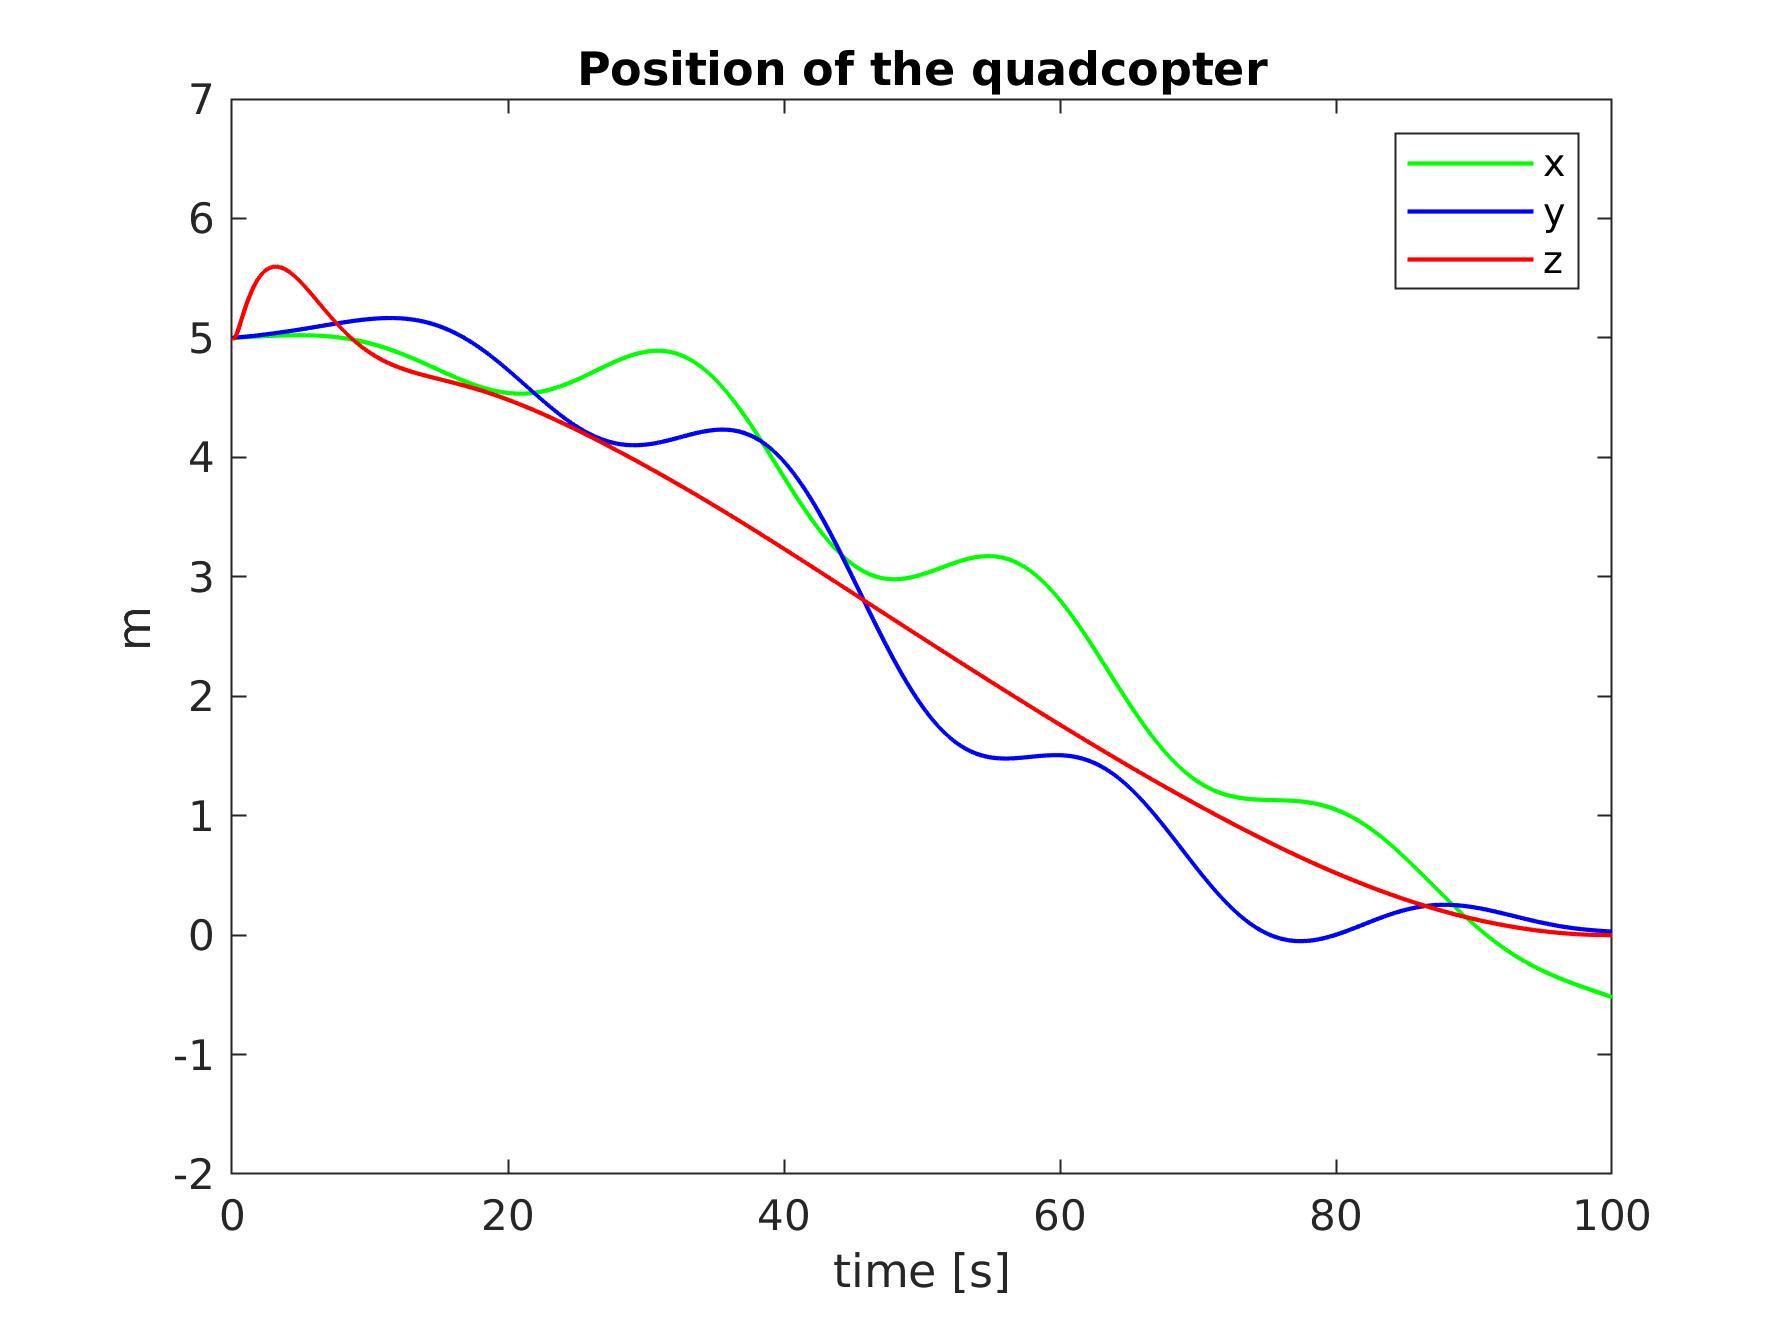
\includegraphics[width=\textwidth]{../report/Images/Position}
\end{frame}

\begin{frame}[fragile]{Complete loop}
  \begin{columns}
    \column{.55\textwidth}
    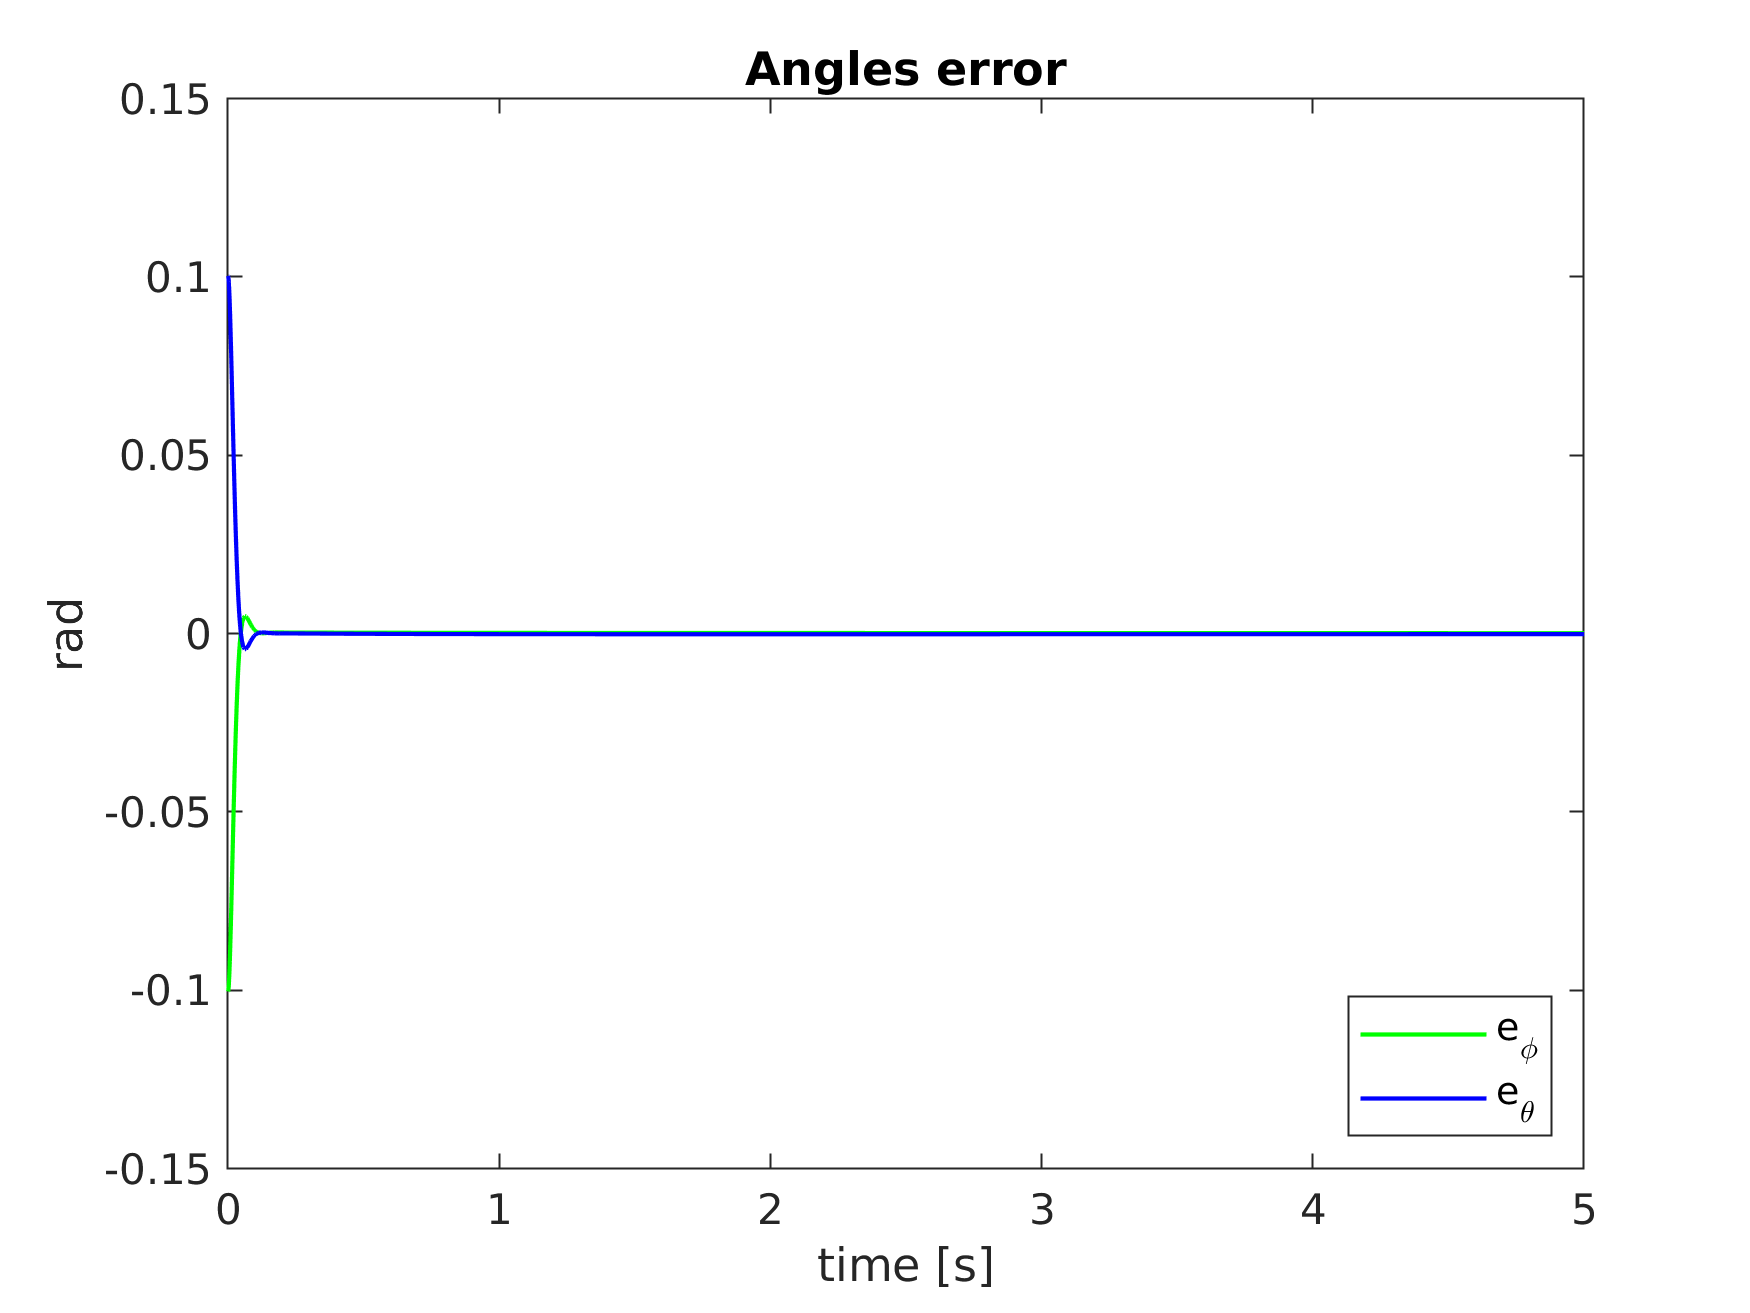
\includegraphics[width=\textwidth]{../report/Images/Angles_error}
    \column{.55\textwidth}
    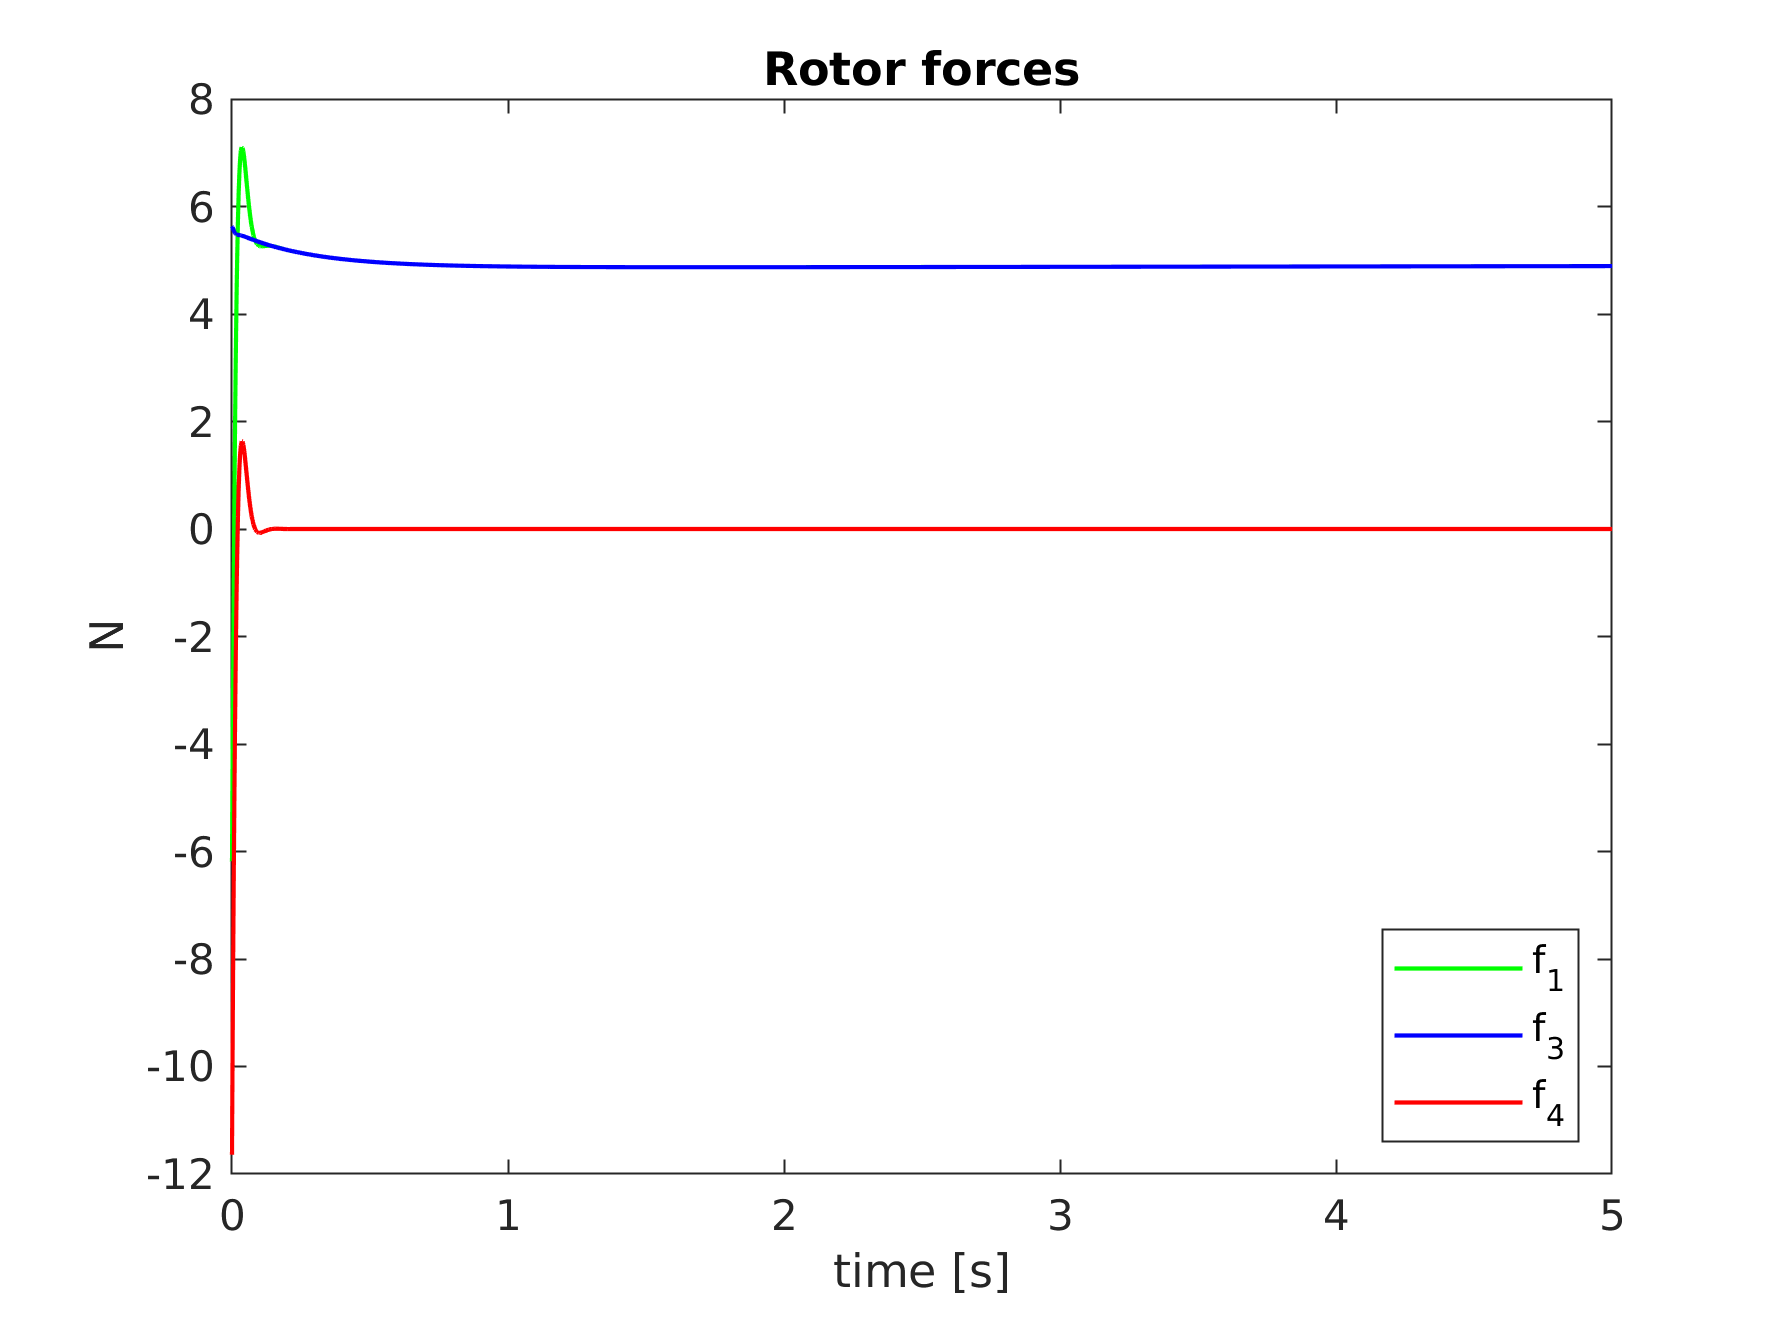
\includegraphics[width=\textwidth]{../report/Images/Forces}
  \end{columns}
\end{frame}

\begin{frame}[fragile]{Complete loop}
  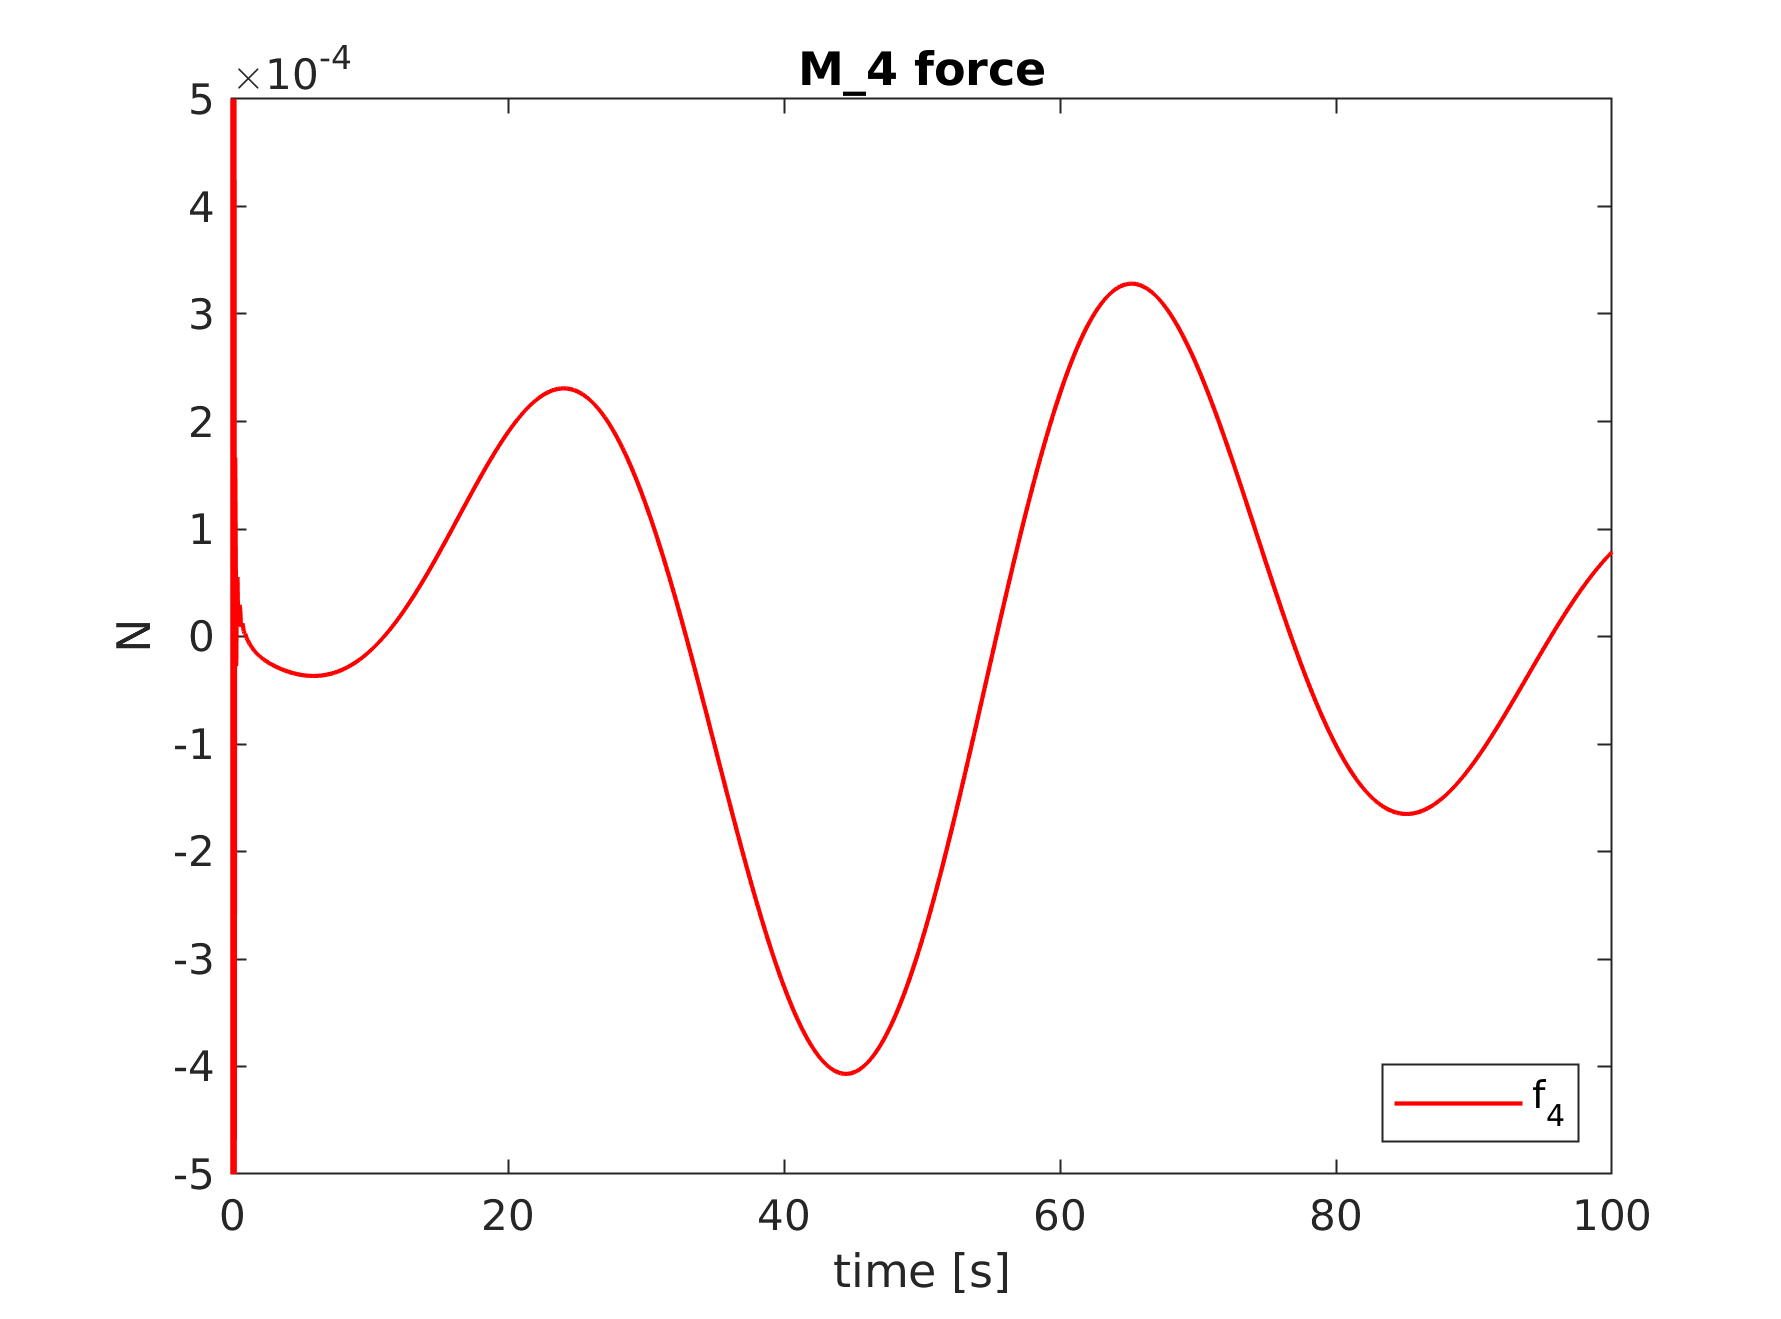
\includegraphics[width=\textwidth]{../report/Images/r4force}
\end{frame}




\section{Conclusions}
\begin{frame}[fragile]{Conclusions }
  \color{LightBlue}
  \textbf{Problem statement:} 
  \color{Black}
  \begin{itemize}
  \item
    Control a quadcopter in case off loss off one of the actuators
  \end{itemize}

  \color{LightBlue}
  \textbf{Proposed solution:}  
  \color{Black}
  \begin{itemize}
  \item
    Adopted strategy: \color{Orange}double loop \color{Black}architecture
  \item
    Sacrified state: yaw angle
  \end{itemize}

  \color{LightBlue}
  \textbf{Consequences:}
  \color{Black}
  \begin{itemize}
  \item
    Horizontal positions oscillates around the desired trajectory, allowing only
    slow recovering manouvers
  \end{itemize}

  \color{LightBlue}
  \textbf{Issues:}
  \color{Black}
  \begin{itemize}
  \item
    Motors force saturation, considered as uncertainty in the model
  \end{itemize}

\end{frame}

